%% Font size %%
\documentclass[11pt]{article}

%% Load the custom package
\usepackage{Mathdoc}

%% Numéro de séquence %% Titre de la séquence %%
\renewcommand{\centerhead}{Chap. 2 : Dérivation (Problèmes de recherche)}

%% Spacing commands %%
\renewcommand{\baselinestretch}{1}
\setlength{\parindent}{0pt}

\begin{document}
\nopagebreak
\begin{exercice}[0][Expérimentations, et Calculs théoriques]
  \begin{center}
    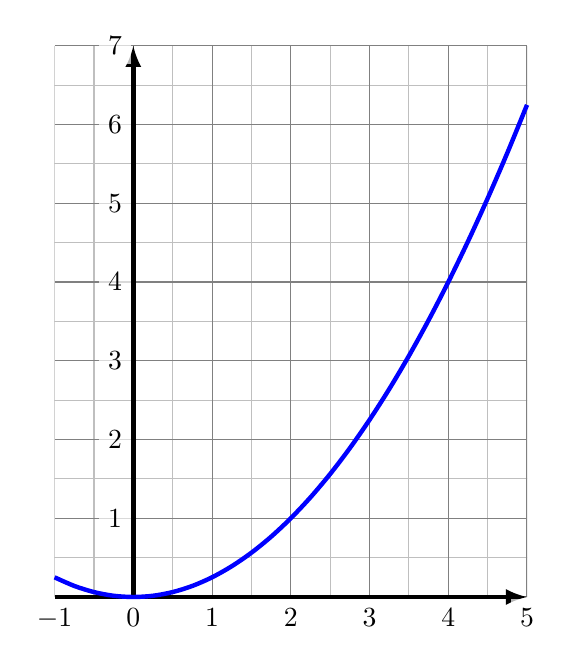
\begin{tikzpicture}[ultra thick, scale=1]
      \begin{scope}
        \clip (-1, 0) rectangle (5, 7);
        \draw[gray!50!white, thin, xshift=-0.5cm, yshift=-0.5cm] (-1, -1) grid (6, 8);
        \draw[gray, thin] (-1, 0) grid (5, 7);
      \end{scope}
      \draw[-latex] (-1, 0) -- (5, 0);
      \draw[-latex] (0, 0) -- (0, 7);
      \foreach \x in {-1, 0, ..., 5} {
        \draw (\x, 0) node[below, fill=white, opacity=.7, text opacity=1]{$\x$};
      }
      \foreach \y in {1, 2, ..., 7} {
        \draw (0, \y) node[left, fill=white, opacity=.7, text opacity=1]{$\y$};
      }

      \draw[domain=-1:5,smooth,variable=\x,blue] plot ({\x},{\x*\x/4});

    %\draw[dashed] (2, 0) node[below]{$x$} -- (2, {2*2/4}) node{$\bullet$} -- (0, {2*2/4}) node[left]{$f\left( x \right)$};
    %\draw[dashed] (3, 0) node[below]{$x+h$} -- (3, {3*3/4}) node{$\bullet$} -- (0, {3*3/4}) node[left]{$f\left( x +h\right)$};
    %\draw[latex-latex] (2, -1) -- (3, -1) node[below, midway]{$h$};
    %\draw[dotted] (1, 0) -- (4, 3);
    \end{tikzpicture}
  \end{center}

  \begin{enumerate}
    \item On a tracé ci-dessus la courbe $\mathcal{C}_f$ de la fonction $f:x\mapsto \frac{x^2}{4}$.
      \begin{enumerate}
        \item Déterminer (par le calcul) l'équation de la tangente à $\mathcal{C}_f$ au point d'abscisse 2. On appelle $d$ la fonction affine correspondante.
        \item Tracer cette tangente.
        \item Calculer $f(x)-d(x)$ pour $x=4$, $x=3$, $x=2,5$, et $x=2,1$.
        \item Vers quelle valeur semble tendre $f\left( x \right)-d\left( x \right)$ lorsque $x$ tend vers 2 ?
      \end{enumerate}
    \item On cherche à résoudre l'équation différentielle :
      \[\left\{\begin{array}{l}
          2f\left( x \right)-xf'\left( x \right)=0\\
          f\left( 2 \right) = 1 \\
      \end{array}\right.\]
      Dans les questions \ref{q:euler:debut} à \ref{q:euler:fin}, on suppose que le tracé correspond \emph{exactement} au tracé de la courbe de la fonction $f$.
      \begin{enumerate}
        \item Isoler $f'\left( x \right)$ dans l'équation précédente.
        \item\label{q:euler:debut} Placer le point de coordonnées $\left( 2; f\left( 2 \right) \right)$.
        \item Calculer $f'\left( 2 \right)$, puis tracer le segment de la droite passant par le point de coordonnées $\left( 2; f\left( 2 \right) \right)$, et de coefficient directeur $f'(2)$, pour $x\in\left[ 2; 3 \right]$.
        \item\label{q:euler:fin} Même question, pour une abscisse de 3, puis de 4.
        \item Vérifier que la fonction $f:x\mapsto\frac{x^2}{4}$ est une solution de l'équation.
        \item Comparer la courbe tracée à cette question, et la courbe de la fonction $f$. Comment faire pour améliorer la précision du tracé ?
          % TODO Faire tracer cette courbe sur un autre graphique, et comparer ensuite les deux courbes
      \end{enumerate}
    \item \emph{Généralisation} Soit $f$ une fonction dérivable, et $a$ un réel de son ensemble de définition.
      On suppose que pour des valeurs de $h$ suffisament petites, $f\left( a+h \right)$ est exactement égale à l'image de $a+h$ par la tangente à $f$ en $a$.
      \begin{enumerate}
        \item Rappeler l'équation de la tangente à $f$ au point d'abscisse $a$.
        \item En déduire l'expression de $f\left( a+h \right)$ en fonction de $f\left( a \right)$, $f'\left( a \right)$ et $h$.
      \end{enumerate}
  \end{enumerate}
\end{exercice}


\end{document}
